\documentclass{article}
\usepackage[spanish]{babel}
\usepackage[utf8]{inputenc}
\usepackage[T1]{fontenc}
\usepackage{graphicx}
\usepackage{listings}
\lstset{language=R, breaklines=true}
\usepackage{amsmath}
\usepackage{subcaption}
\usepackage[left=4cm,right=4cm]{geometry}
\usepackage[numbers,sort&compress]{natbib}


\title{\bf Práctica 11: frentes de Pareto}
\date{\today}
\author{C. A. Estrada}

\begin{document}

\maketitle

\section{Objetivo}
Graficar el porcentaje de soluciones de Pareto \cite{dra}, como función del número de funciones objetivo $k$ con diagramas de violín combinados con diagramas de caja-bigote, verificando si existen diferencias significativas.

\section{Metodología}
Se emplea el paquete estadístico R versión 4.0.2 \cite{R} para la generación del código, utilizando lo previamente reportado para el frente de Pareto \cite{dra}. Para ello, se emplean desde 2 hasta 12 funciones objetivo, y se anida el código en dos ciclos "for", uno para las funciones objetivo a utilizar, y otro para las réplicas, de las cuales se utilizan 20.
\begin{lstlisting}
vc =4
md = 3
tc = 5
fo = seq(2, 12, by=1) 
resultados=data.frame()
for (k in fo){
  for(rep in 1:20){
\end{lstlisting}
Al finalizar los ciclos, se obtiene el porcentaje de soluciones de Pareto.
\begin{lstlisting}
frente = subset(val, no.dom) 
porcentaje=(sum(no.dom)/n)*100 
resultados=rbind(resultados, c(k, rep, porcentaje))
\end{lstlisting}

Finalmente, se genera un gráfico con diagramas de violín combinados con diagramas de caja-bigote empleando el paquete \textit{ggplot2} \cite{gg}, y se verifican las diferencias estadísticas mediante las pruebas de Kruskal-Wallis y Mann-Whitney para cada par de grupos.

\section{Resultados y discusión}
En la figura \ref{box} se presentan los porcentajes de soluciones de Pareto obtenidos durante la ejecución del experimento. Se puede observar una clara tendencia al aumento de las soluciones no dominadas conforme se incrementa el número de funciones objetivo, en donde llega hasta casi $100\%$ para el caso en donde se emplean 12 funciones objetivo. Por lo tanto, de acuerdo con estos resultados, en una optimización multicriterio, el utilizar más de 6 funciones objetivo no sería recomendable.

\begin{figure}[ptb]
\begin{center}
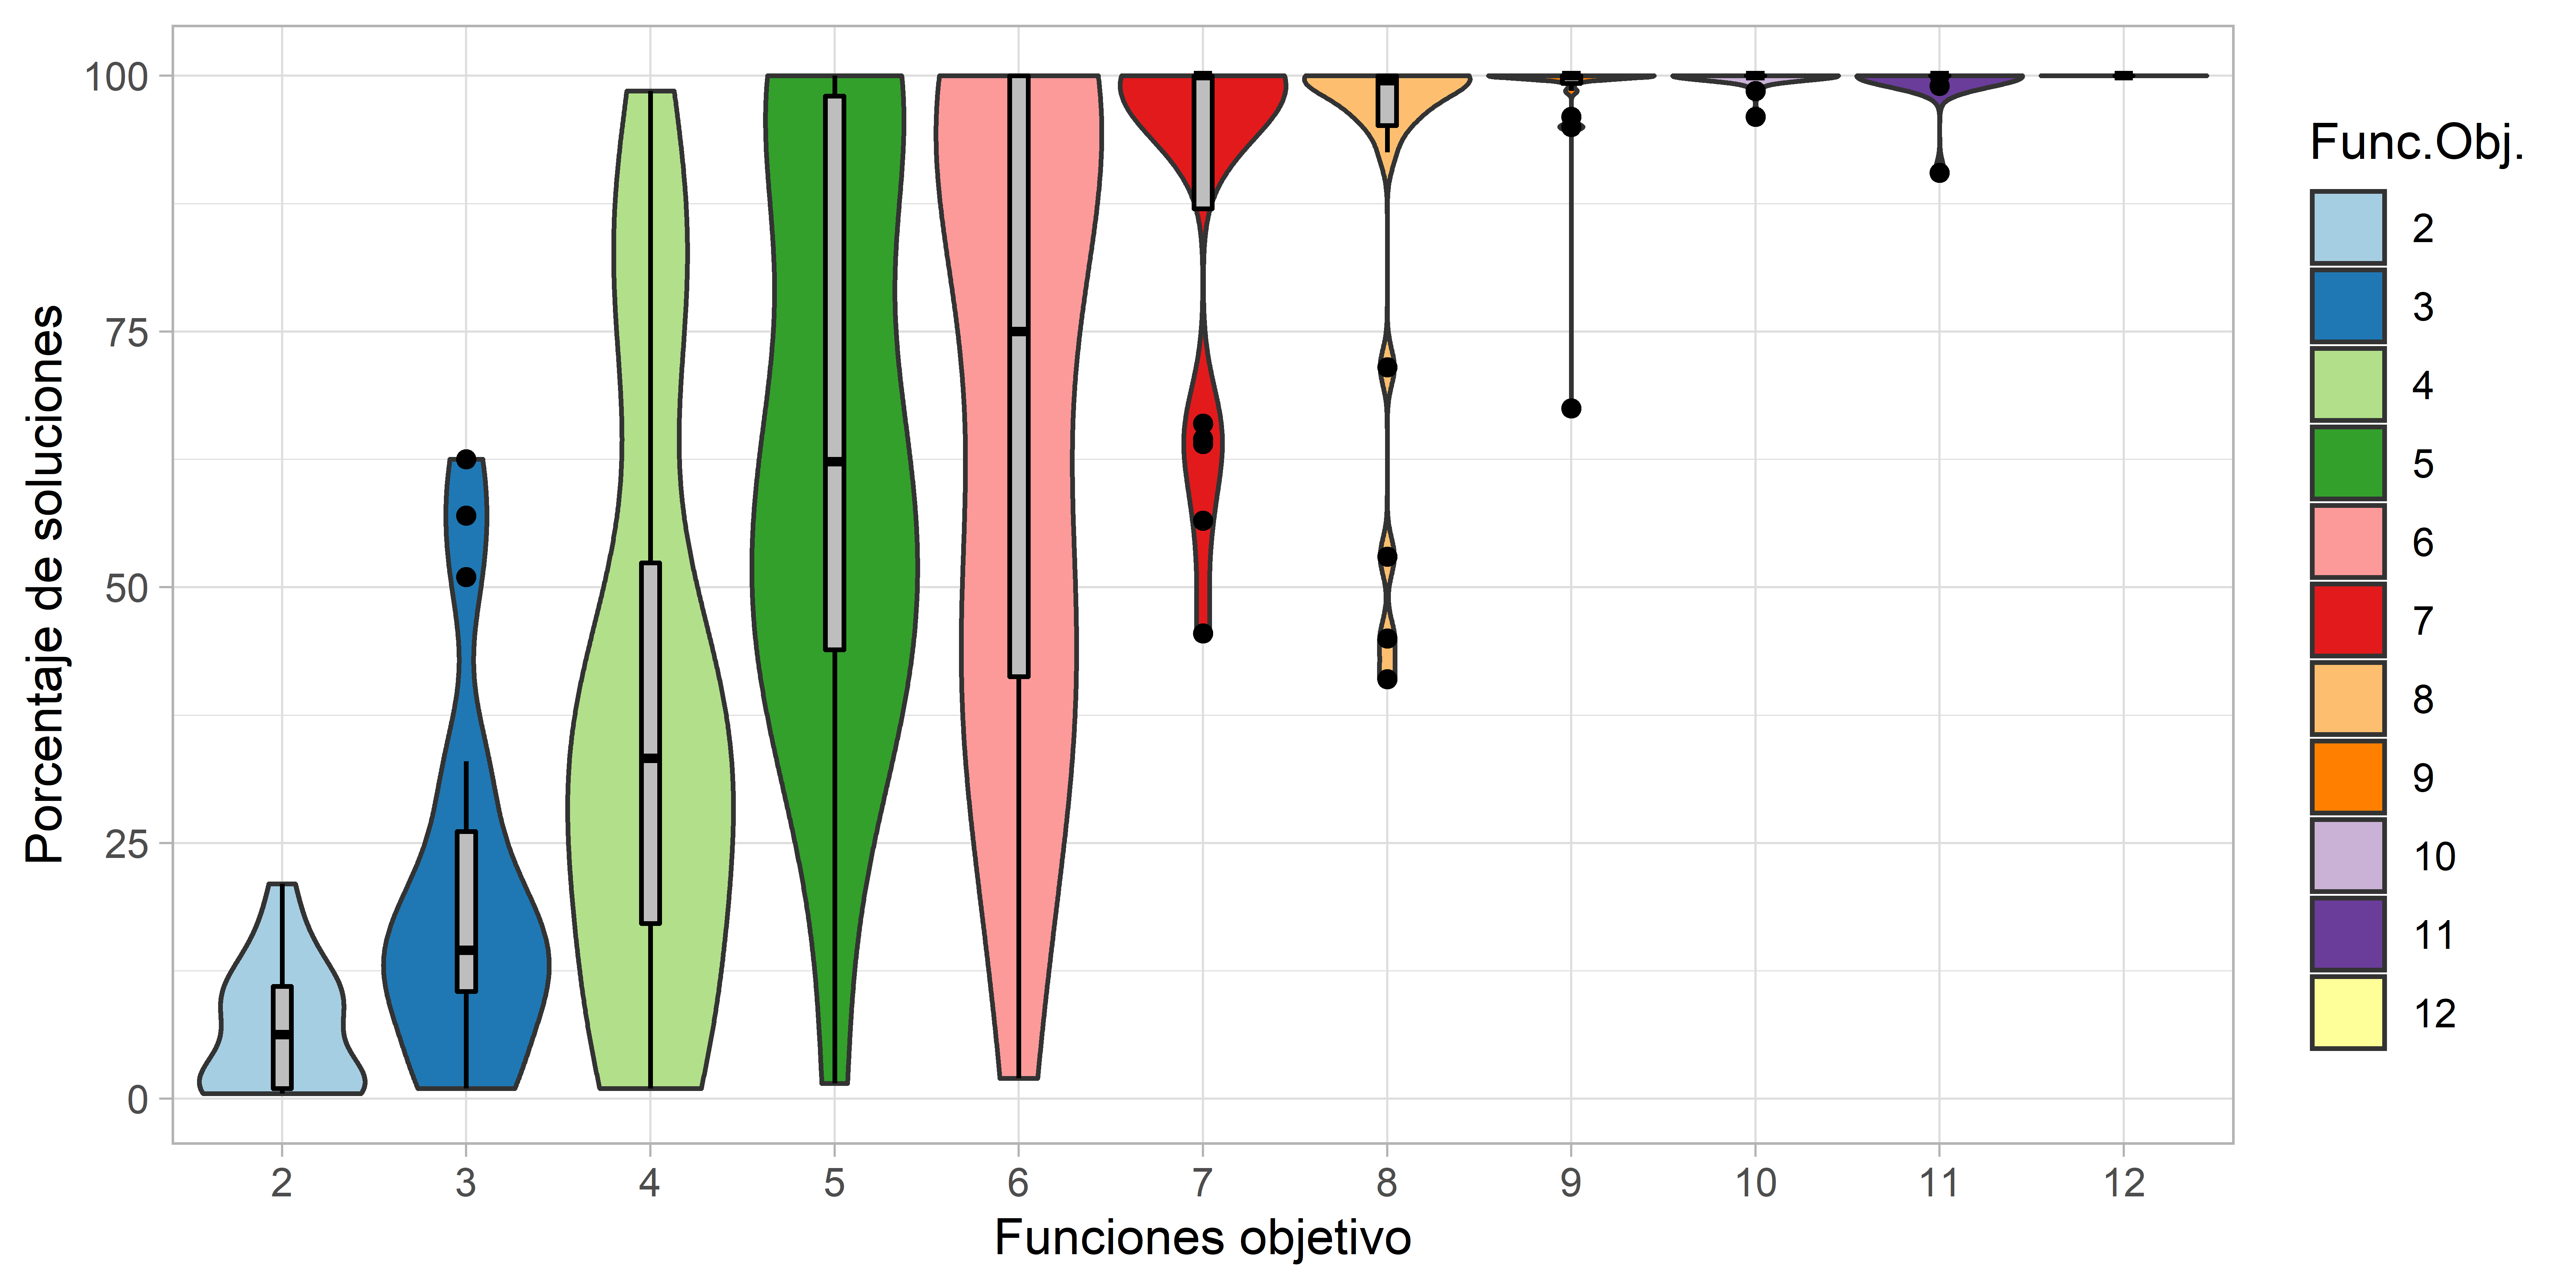
\includegraphics[width=\linewidth]{p11.png}
\end{center}
\caption{Porcentaje de soluciones de Pareto no dominadas para diferentes cantidades de funciones objetivo ($k$).\label{box}}
\end{figure}

Para verificar diferencias estadísticas, se emplea primeramente la prueba de Kruskal-Wallis tomándose una significancia de 0.05, en donde el valor $p$ obtenido es de $<2.20\times10^{-16}$, por lo que se rechaza la hipótesis nula, indicando que existen diferencias significativas entre al menos alguno de los grupos estudiados. Por ende, se realiza la prueba de Mann-Whitney para cada par de grupos estudiados, cuyos resultados se presentan en el cuadro \ref{mw}. Tomando, de igual forma, una significancia de 0.05, se observa que existen diferencias significativas para la mayoría de las funciones objetivo, excepto para los valores más altos, es decir, cuando se utilizan 9, 10, 11 y 12 funciones objetivo.

\begin{table}[h]
\begin{center}
\caption{Comparación de cada par de grupos de las funciones objetivo mediante la prueba de Mann-Whitney.}
\label{mw}
\tabcolsep=0.11cm
\small
\begin{tabular}{r r r r r r r r r r r}
\hline
 &\textbf{2}&\textbf{3}&\textbf{4}&\textbf{5}&\textbf{6}&\textbf{7}&\textbf{8}&\textbf{9}&\textbf{10}&\textbf{11}\\
\textbf{3}&0.03337& & & & & & & & & \\
\textbf{4}&0.00158&0.43781& & & & & & & & \\
\textbf{5}&1.6e-05&0.00062&0.11554& & & & & & & \\
\textbf{6}&1.5e-05&0.00075&0.10076&1.00000& & & & & & \\
\textbf{7}&2.1e-06&4.4e-06&0.00013&0.10347&0.30278& & & & & \\
\textbf{8}&2.3e-06&7.1e-06&9.9e-05&0.11701&0.35699&1.00000& & & & \\
\textbf{9}&1.6e-06&1.6e-06&5.3e-06&0.00279&0.02762&1.00000&1.00000& & & \\
\textbf{10}&7.7e-07&7.7e-07&9.1e-07&0.00018&0.00165&0.12172&0.10076&0.97223& & \\
\textbf{11}&7.7e-07&7.7e-07&8.6e-07&0.00018&0.00165&0.13563&0.10347&1.00000&1.00000& \\
\textbf{12}&4.3e-07&4.3e-07&4.3e-07&4.1e-05&0.00030&0.02233&0.01002&0.13406&1.00000&1.00000\\
\hline
\end{tabular}
\end{center}
\end{table}

\section{Conclusión}
El porcentaje de soluciones de Pareto no dominadas aumenta conforme se incrementa el número de funciones objetivo, con diferencias significativas entre la mayoría de los grupos.

\section{Reto 1}
Se pretende seleccionar un subconjunto del frente de Pareto de tal forma que la selección esté diversificada \cite{dra}, y posteriormente, graficar los resultados de la selección, indicando con distinto color los que pertenecen al subconjunto.
Para ello, se toma el código base para la generación del frente de Pareto \cite{dra,ric} y se selecciona el $60\%$ del frente.
\begin{lstlisting}
frente = subset(val, no.dom) 
p=0.6
subconjunto=frente[c(round(runif(round(dim(frente)[1]*p), min = 1, max = dim(frente)[1]))),]
\end{lstlisting}

Posteriormente, se genera el gráfico, como se presenta en la figura \ref{sub}, en donde se observa el subconjunto del frente de Pareto seleccionado como puntos morados, mientras que el frente original se compone de los puntos color rosa.

\begin{figure}[ptb]
\begin{center}
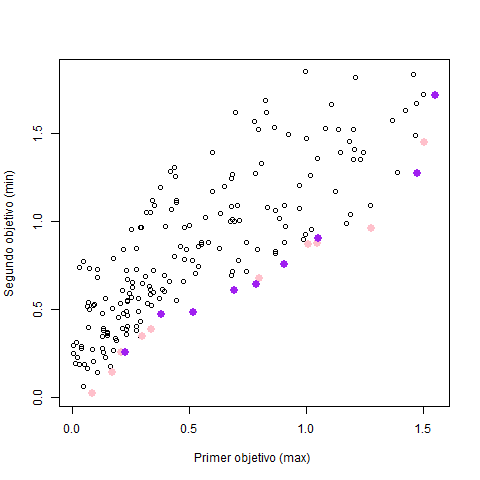
\includegraphics[width=\linewidth]{p11-sub.png}
\end{center}
\caption{Subconjunto del frente de Pareto seleccionado, en donde los puntos de color morado pertenecen al subconjunto y los de color rosa al frente original.\label{sub}}
\end{figure}

\bibliography{P11}
\bibliographystyle{unsrtnat}

\end{document}